%\pagenumbering{arabic}%start arabic pagination from 1 

\chapter{Praktická část}

popis

\section{Návrh}

test

\subsection{Cíle aplikace}

\begin{itemize}
\item Přidání a odstranění jednotlivých bodů v MindMapě
\end{itemize}

\section{Základní aplikace}

Spuštění verticle programově
\begin{lstlisting}
JsonObject config = new JsonObject();
config.putString("foo", "wibble");
config.putBoolean("bar", false);
container.deployVerticle("foo.ChildVerticle", config);
\end{lstlisting}

Spuštění verticle z příkazové řádky
\begin{lstlisting}
vertx run foo.js -conf myconf.json
\end{lstlisting}

\section{Integrace s databází MongoDB}

databaze

\section{Komunikace v reálném čase}\label{sec:realTimeCommunication}

\begin{figure}
\begin{centering}
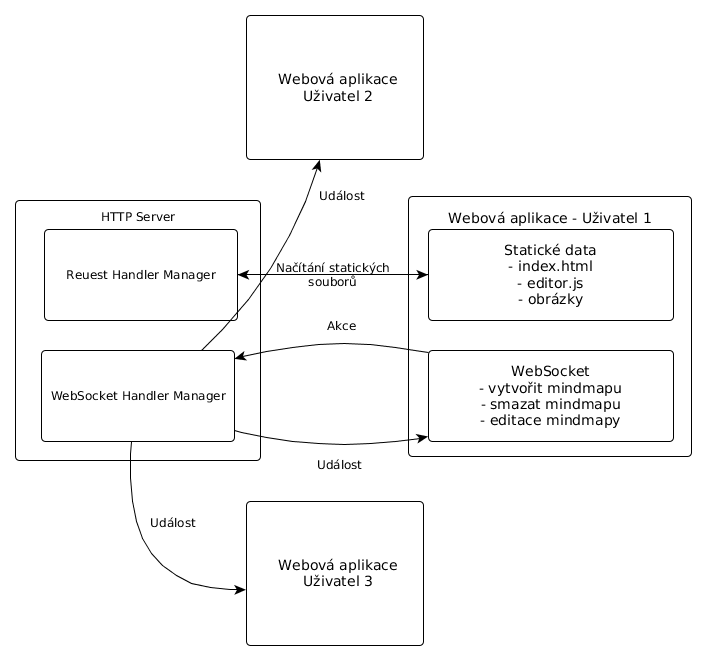
\includegraphics[width	=1\textwidth]{obrazky/realtime_communication}
\par\end{centering}
\caption{Komunikace v reálném čase\label{fig:realtime_communication}}
\end{figure}

\section{Polyglot vývoj a moduly}\label{sec:praktickyModuly}

 deskriptor\emph{toto je poze základní výčet parametrů všechny lze nalézt v dokumentaci Vert.x}

\begin{lstlisting}
{
  "main": "EchoServer.java",
  "worker": true,
  "includes": "io.vertx~some-module~1.1",
  "auto-redeploy": true
}
\end{lstlisting}

Parametr \emph{auto-redeploy} mluví sám za sebe.

Jak bylo řečeno v \ref{sub:hybrid} Vert.x instance má dvě sady vláken. Parametrem \emph{worker} v deskriptoru modulu, lze říci Vert.x jádru aby spustil modul v \emph{background worker poolu}. 

Spuštění modulu programově v jazyce Java
\begin{lstlisting}
container.deployModule("io.vertx~mod-mailer~2.0.0-beta1", JSONconfig);
\end{lstlisting}

Spuštění modulu z příkazové řádky
\begin{lstlisting}
vertx runmod com.mycompany~my-mod~1.0 -conf config.json
\end{lstlisting}

moduly vice jazyku

\section{Nasazení}

deploy + scaling

\subsection{Server}

ubuntu

\subsection{Java}

java

\subsection{Vert.x}

vert.x

\subsection{MongoDB}

mongodb

\section{Škálování a vysoká dostupnost}\label{sub:Scaling}

možnosti škálování a HA

\subsection{Počet Verticlů}
verticle count

\subsection{Vert.x v clusteru}\label{sub:praktCluster}
HA
